\documentclass[12pt]{standalone}
\usepackage{amsmath, relsize, tikz}
\usepackage{xcolor}
\usepackage{pgffor} % LATEX
\input pgffor.tex % plain TEX
\usetikzlibrary{matrix}
\usetikzlibrary{knots}  
\usetikzlibrary{intersections,backgrounds}
\begin{document}
    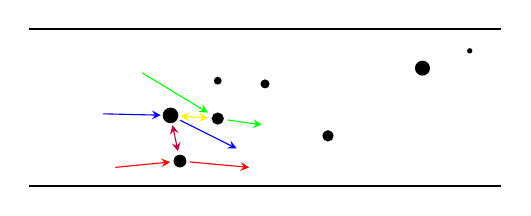
\begin{tikzpicture}[scale=2.0, >=stealth]
%        \draw [lightgray, thin, step = 0.5] (0,0) grid +(3,1);
%        \draw [step = 1] (0,0) grid +(10, 10);
%        \draw [blue, ultra thick] (0, 0) rectangle (10, 10);
%        \draw [red] (2.5, 0) .. controls +(right:1) and +(right:1) .. (2.5, 1);

%        \foreach \y in {0.1, 0.2, ..., 0.9}
%        {
%            \draw [blue, ->] (-0.2, \y) -- (0.2, \y);
%            \draw [blue, ->] (12.9906 *\y - 83.2617 *\y^2 + 277.778 *\y^3 - 481.978 *\y^4 + 411.706 *\y^5 - 137.235 *\y^6 + 2.0, \y) --
%                             (12.9906 *\y - 83.2617 *\y^2 + 277.778 *\y^3 - 481.978 *\y^4 + 411.706 *\y^5 - 137.235 *\y^6 + 2.5, \y);
%        }


        \draw [thick] (0, 1) -- (3, 1);
        \draw [thick] (0, 0) -- (3, 0);
%
        \foreach \i/\x/\y/\size in
        {
            1/0.90/0.45/0.046,
            2/0.96/0.16/0.037,
            3/1.50/0.65/0.025,
            4/2.80/0.86/0.013,
            5/1.20/0.67/0.021,
            6/1.90/0.32/0.032,
            7/2.50/0.75/0.044,
            8/1.20/0.43/0.035
        }
        {
            \draw [fill] (\x, \y) circle [radius=\size] node (\i) {};
        }
        \draw [blue, ->] (0.47, 0.46) -- (1);
        \draw [blue, ->] (1) -- (1.32, 0.24);

        \draw [purple, <->] (1) -- (2);
        \draw [yellow, <->] (1) -- (8);

        \draw [red, ->] (0.55, 0.12) -- (2);
        \draw [red, ->] (2) -- (1.40, 0.12);


        \draw [green, ->] (0.72, 0.72) -- (8);
        \draw [green, ->] (8) -- (1.48, 0.39);
%        \node [below] at (10, 0) {1.0};
%        \node [left] at (0, 10) {1.0};
%        \draw (0, 0) -- (1, 0) -- (0.5, 0.866) -- cycle;
%
%        \draw [fill] (0, 0) circle [radius=0.025];
%        \node [below left] at (0, 0) {$p_i$};
%        \draw [fill] (1, 0) circle [radius=0.025];
%        \node [below right] at (1, 0) {$p_{i+1}$};
%        \draw [fill] (0.5, 0.866) circle [radius=0.025];
%        \node [above] at (0.5, 0.866) {$p_{i+2}$};
%
%        \node [below] at (0.5, 0.433) {\huge $e_j$};
    \end{tikzpicture}
\end{document}
